\chapter{MATERIALS AND METHODS} \label{chapter:materials_methods}
    \section{Proposed System} \label{sec:proposed_system}
    The general idea was to create a system that would be able to provide accompaniment to a human soloist, based on given lead sheet chords, in real time. The system's task is to interpret the information given from the lead sheet with variability, depending on the predicted harmonic variability of the human solo. In order for the system to do so, data need to include information about the following:
    
    \begin{itemize}
        \item Metric structure
        \item Human solo channel
        \item Accompaniment channel
        \item Lead sheet information
    \end{itemize}
    
    Providing the system with all the information above, it will have the ability to recognise measure changes, respond to the expected human solo and learn to comply with the given lead sheet chords, resulting in producing proper accompaniment for the human solo.

    \section{Data Preprocessing}
    Due to the lack of a readily available dataset that includes all of the information above, a need of such emerged. This section describes the exact procedures that were followed, $e.g.$ modification and augmentation of the original dataset, to create a proper dataset for the task of the system training.

        \subsection{Description of the dataset} \label{subsec:initial_dataset}
        The initial dataset\footnote{\url{https://github.com/wayne391/lead-sheet-dataset/} -- last accessed October 27 2019.} \cite{liu2018lead}, carries information about the pieces that are included -- the tempo, beat, melody and chords on the lead sheet. The beat information indicates the measure structure. One time-stamp corresponds to 1/24 of a quarter note, a time resolution able to represent rhythm values of even sixty-fourth triples. The melody and the accompanying chords are saved as 128-keys piano roll representations with the time resolution mentioned above, where the note that is played at each time-step, is indicated by its velocity value. However, following this type of representation, a possible note repetition cannot be clear, as there is not a way to distinguish one single quarter (note or chord) held for 24 time steps, from two successive eighths (notes or chords) each one held for 12 time steps. 

        \subsection{Time Resolution} \label{subsec:time_resolution}
        The time resolution was reduced, from 24 time-steps per beat(quarter) to 2 steps per beat, in order for each time-stamp to represent an eighth note, which is half the duration of the quarter. To perform this task, from each beat that lasts 24 time-steps, only the information that is indicated by the first and the thirteenth step is kept. More specifically, the followed procedure involves splitting each quarter in half, in order to create two subsets of 12 time-steps each and then keeping only the first step of each subset. As a result, the initial quarter was replaced by two eighths, with a new resolution of 2 instead of 24 time-steps each.
        
        \subsection{Chord Information} \label{subsec:chord_info}
        For the proposed system's training, chord information needs to be represented in a new, more useful for the purpose of the research and compact way, in the form of lead sheet for jazz standards. To do so, the accompanying chords channel information given by initial dataset are used. Specifically, instead of the velocity values of the active notes that compose the chord at each time-step and their respective midi numbers, only the pitch class of the chords' root is kept, as well as the chord type, with the help of ready-made functions from the MIT Music21 Python library\footnote{\url{https://web.mit.edu/music21} -- last accessed October 27 2019.}, a toolkit for computer-aided musicology. This library, contains functions capable of multiple operations, such as chord information extraction, construction of musical elements and score/music stream creation, employing raw data. In detail, for the construction of this new information representation needed, a 12-sized vector containing the root pitch class information is stacked with 3 vectors of size 2, containing chord type information about major/minor 3rd, perfect/augmented/diminished 5th and major/minor 7th, respectively. The reason behind this specific kind of chord information representation on the lead sheet, is the fact that jazz musicians need a fundamental description of harmony, that gives them the freedom to perform creatively, by being able to make alterations to each musical piece. The types of chords that the employed scheme is able to represent are the basic, e.g. major/minor triads, dominant/7, major 7th, half(diminished) and augmented.
        
        \subsection{Data Augmentation}
        As mentioned above, the initial dataset does not include materialised accompanying chords. To construct them, an algorithm to perform basic harmonic enrichment on the lead sheet chords was created, where they are materialised into actual accompanying chords, with multiple inversions and diverse rhythmic patterns. First, accompaniment chords are assigned to the positions of the lead sheet chord symbols. Then, chords with inversions are placed just after those positions, depending on probabilistic methods, related to the time-steps passed without any chords (it becomes more probable to insert an inverted chord the more time passes) as well as the presence of a note at the melody channel at the respective step of chord (the occurrence of a melodic event, increases the probability of insertion). The purpose of the augmentation of the data, is to enhance the variability in the accompaniment channel, depending on the lead sheet chord symbols and the melodic rhythm patterns.

        \subsection{Transposition}
        To reduce the dependency of the chord progression from the key of the piece which they are part of, the pieces in the dataset were transposed to all the 12 keys. This process, results in greater accuracy of the trained system's predictions on new, unseen data, as it learns to recognise the relative separations between the chords. For example, in cases where a chord sequence in the training or the validation set has already been encountered in the training set but in a different key, the system would be able to predict that chord progression in the test set with high accuracy.
            
        \subsection{Feature Dimensionality Reduction}
        In the melody information channel, each note is represented by a 128-sized vector, as mentioned in section \ref{subsec:initial_dataset} above. This feature, undergoes dimensionality reduction, by flattening each note's vector into a single (the melody channel is monophonic) non-zero value – the midi number of that note. In order to flatten the accompaniment feature, a dictionary of all the unique chords of this channel was created, with each chord been represented by its index in the aforementioned dictionary. The system's purpose is to learn those notes, which means being able to predict the most accurate class (one of all the chords in the dictionary --classification) for this specific time-step of prediction. Those two features' dimensionality reduction (flattening), allows one-hot representation for both data streams (melody and accompaniment). 
        
        
        \subsection{Dictionary Information} \label{subsec:dict_info}
        Before the harmonic enrichment process of the data, the dictionary of the accompaniment chords contained 476 chords, after the augmentation and before the transposition to all the 12 pitches, the classes were 847 and finally, after all the data preparation (after both augmentation and transposition), the number of unique accompaniment chord classes was 2677 .

        %\subsection{MUSIC21} \label{subsec:music21}
        %As mentioned above, in subsection \ref{subsec:chord_info}, Music21\footnote{\url{https://web.mit.edu/music21} -- last accessed October 27 2019.} is a Python library developed by MIT, containing multiple functions that allow computer-aided musicology oriented operations, on raw musical data.

    
    \section{System Architecture}
    The system proposed, consists of two main layers of information processing, one for predicting the next steps of expected human solo and one for producing the final accompaniment chords.
        
        \subsection{Overall Structure} \label{subsec:overall_structure}
        As mentioned above, the accompaniment predictions of the system have to be closely related to the expected human solo of the future time-steps. More specifically, at each step of the prediction process, the information about the intentions of the human soloist at the the upcoming step is needed to predict the accompaniment chord for that specific future step. 
        The predictions are dependent of the past 16 time-steps (16 eighths). Therefore, the data that the system is fed at each iteration to make the respective predictions, are represented as a 16-steps window, comprising the following futures:
        \begin{itemize}

            \item   Metric information ( $b\textsubscript{t}$ )
            \item   Human solo part ( $h\textsubscript{t}$ )
            \item   Accompaniment chords part ( $a\textsubscript{t}$ )
            \item   Lead sheet chord information constructed in subsection \ref{subsec:chord_info} ( $c\textsubscript{t}$ )
            
        \end{itemize}

        The input data windows are overlapping, that means for successive iterations, the respective windows slide one step each time, which is an eighth for the time resolution of the final form of data (detailed explanation on the chosen time resolution in subsection \ref{subsec:time_resolution}).
        
        The system consists of two subsystems, the Human Agent (HA) and the Artificial Agent (AA), to perform the predictions of the human solo and the accompaniment chords respectively. Both of them rely on models that deploy LSTM RNNs, NN architecture explained in subsection \ref{subsec:lstm}, preferable for their effectiveness on models handling sequential data.
        
        \begin{figure}[h]
        \centering
        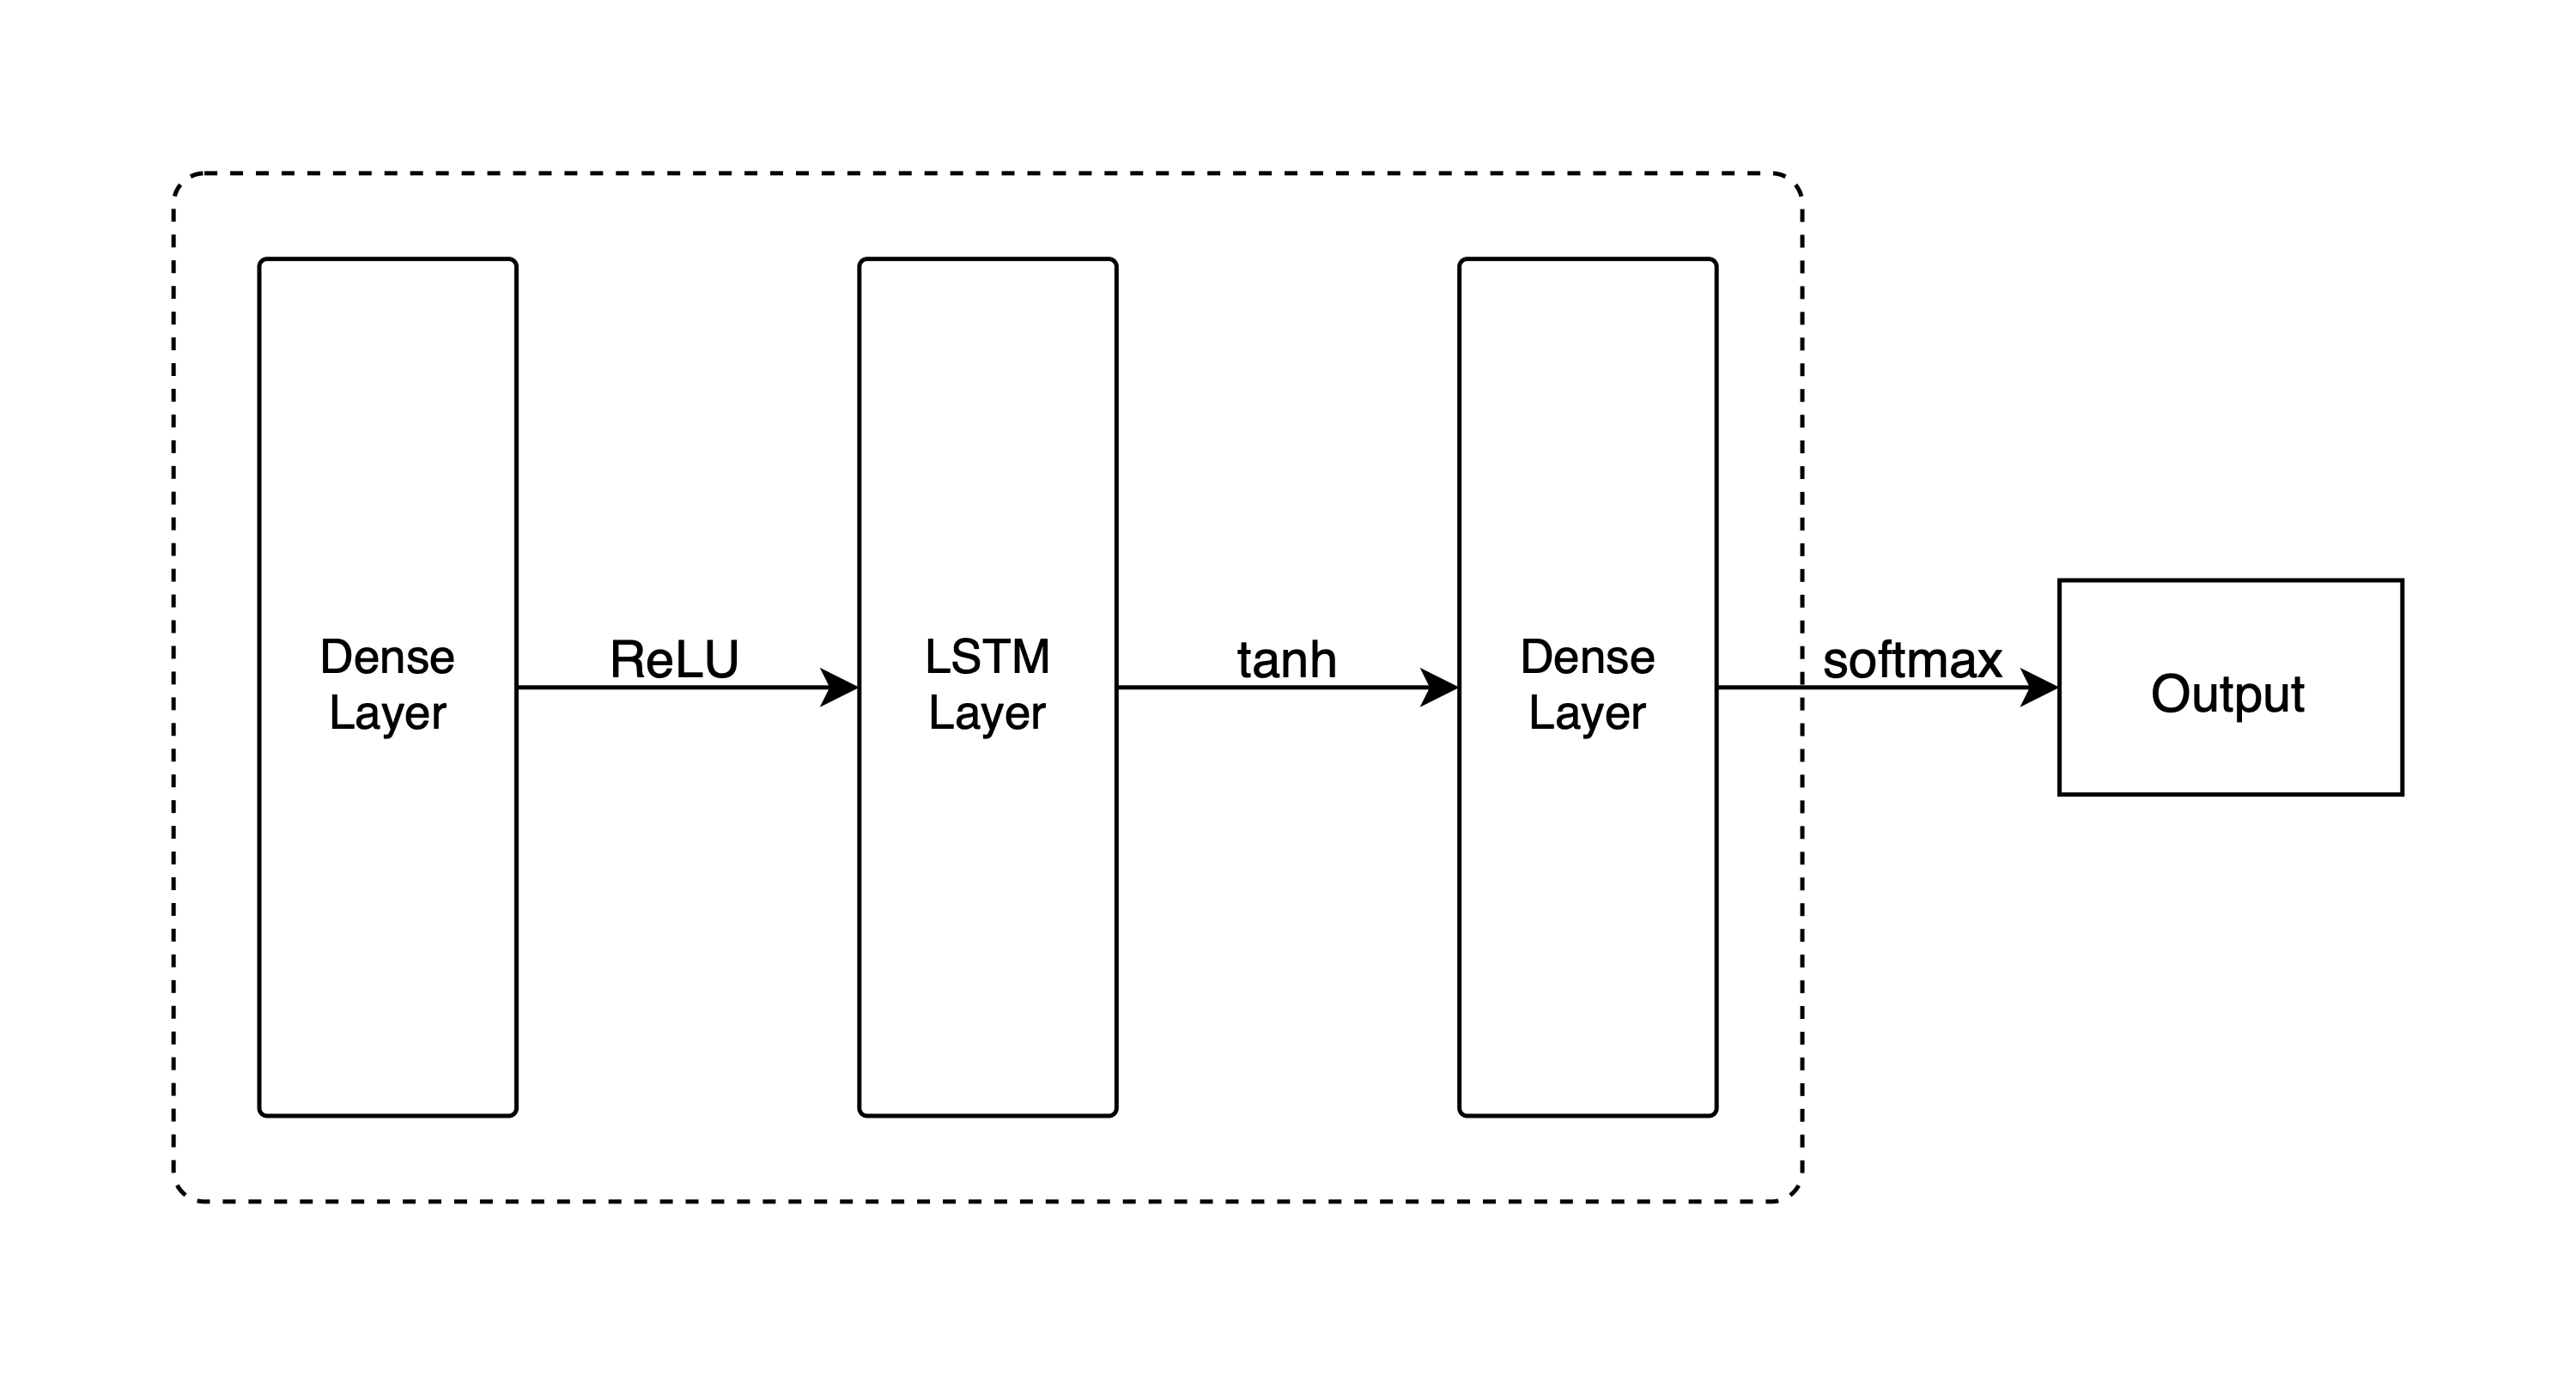
\includegraphics[width=1\textwidth]{media/overall_layers_with_funs.jpg}
        \caption{The architecture of both subsystems}
        \label{fig:system_architecture}
        \end{figure}
        

        The exact model architecture of the system is depicted in figure \ref{fig:system_architecture}. As in figures \ref{fig:ha_architecture} and \ref{fig:aa_architecture}, the input time frame(window) is fed to the two sub-systems, which have the same layer structure, as follows:
        \begin{itemize}
            \item \textbf{DENSE} layer with ReLU activation function
            \item \textbf{LSTM} layer containing 64 cells, using hyperbolic tangent activation function
            \item \textbf{DENSE} layer with softmax activation function
        \end{itemize}
        

        The input frame, first undergoes a linear transformation through the bottom Dense layer, then it is encoded into a latent space through the LSTM layer and finally through the top Dense layer a linear transformation is applied, to a space of the dimensionality of the respective target classes. Here, the softmax activation function as described in subsection \ref{subsec:activation_funs}, results in probabilistic outputs. The final prediction of each of the two subsystems would be the class with the highest probability.

        \subsection{Human Agent (HA)}
        The human agent predicts the human solo of the following step ($h\textsubscript{t+1}$ ) at each time-step $t$, as mentioned above. For this task, the HA's input data windows during the iterative process of successive predictions, include the expected human solo part that this sub-system learns to predict and the metric and lead sheet information channels which are one eighth ahead of the human solo. The accompaniment chords feature is excluded from the HA input. The output of this system, is single-step human solo information (the expected intentions of the soloist) -- one of the 128 possible piano-roll midi numbers, which will then be fed to the AA system as part of the input data window at each iteration.

        \begin{figure}[h]
        \centering
        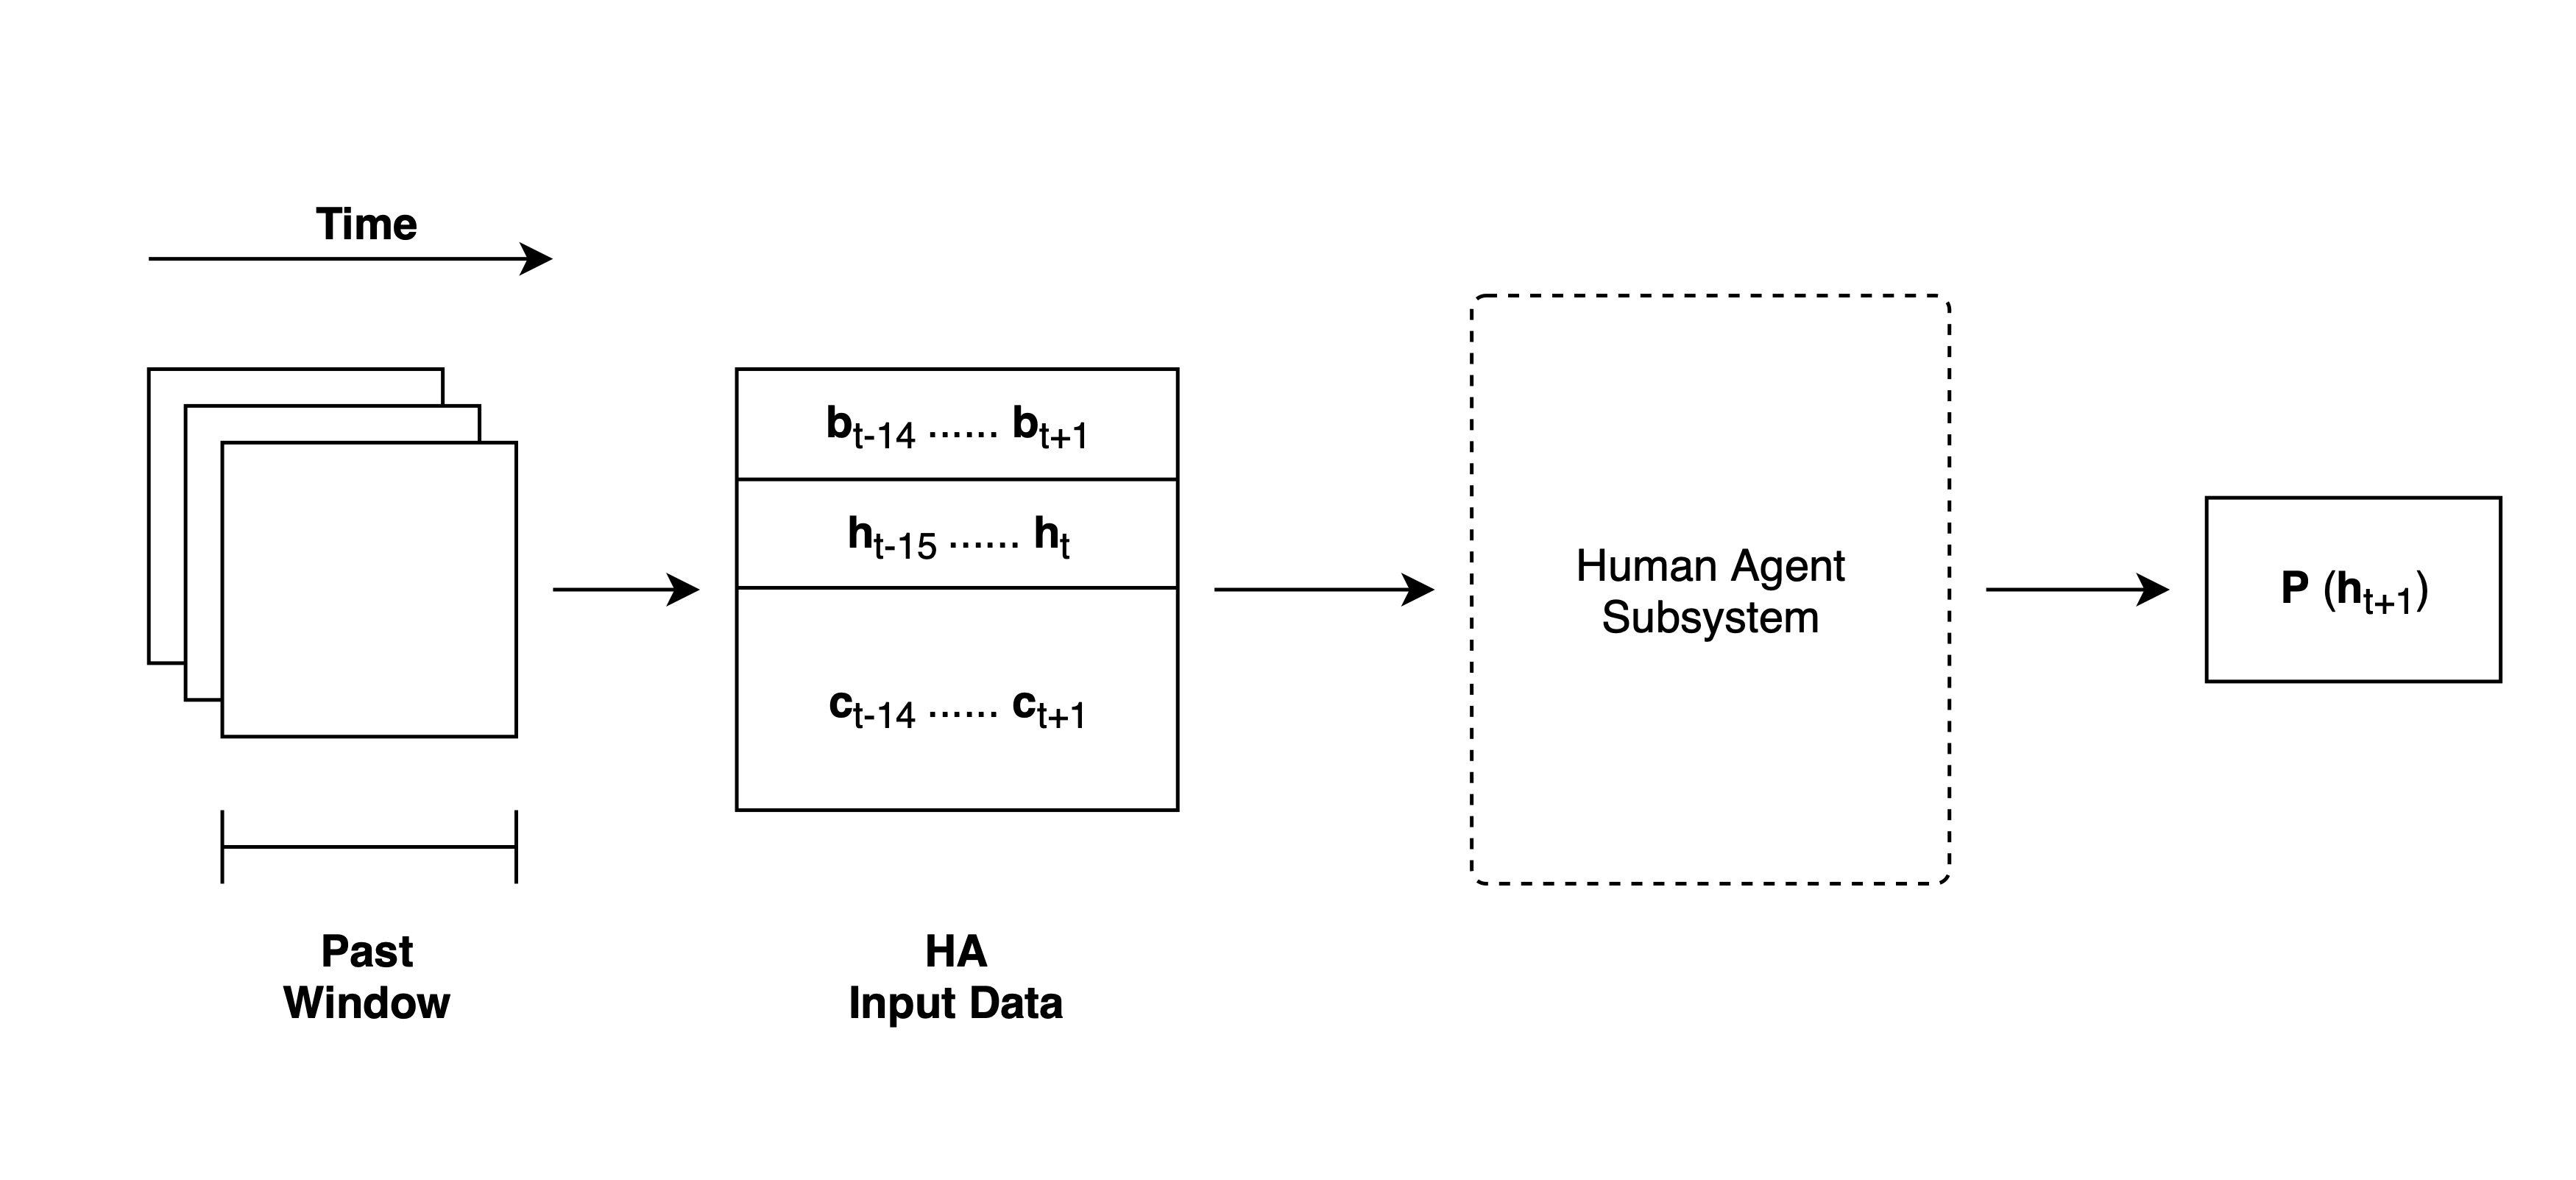
\includegraphics[width=0.8\textwidth]{media/ha_overall.jpg}
        \caption{The Human Agent Subsystem}
        \label{fig:ha_architecture}
        \end{figure}
        
        \subsection{Artificial Agent (AA)}
        The artificial agent, accordingly, predicts the accompaniment chord of step $t+1$ at each step $t$. This sub-system is dependent of all the data information channels, in contrast with the HA, therefore the input data windows during the prediction process, contain all the features mentioned in subsection \ref{subsec:overall_structure}. The AA's output is one of the dictionary's total accompaniment chord classes (dictionary construction details in subsection \ref{subsec:dict_info}).

        \begin{figure}[h]
        \centering
        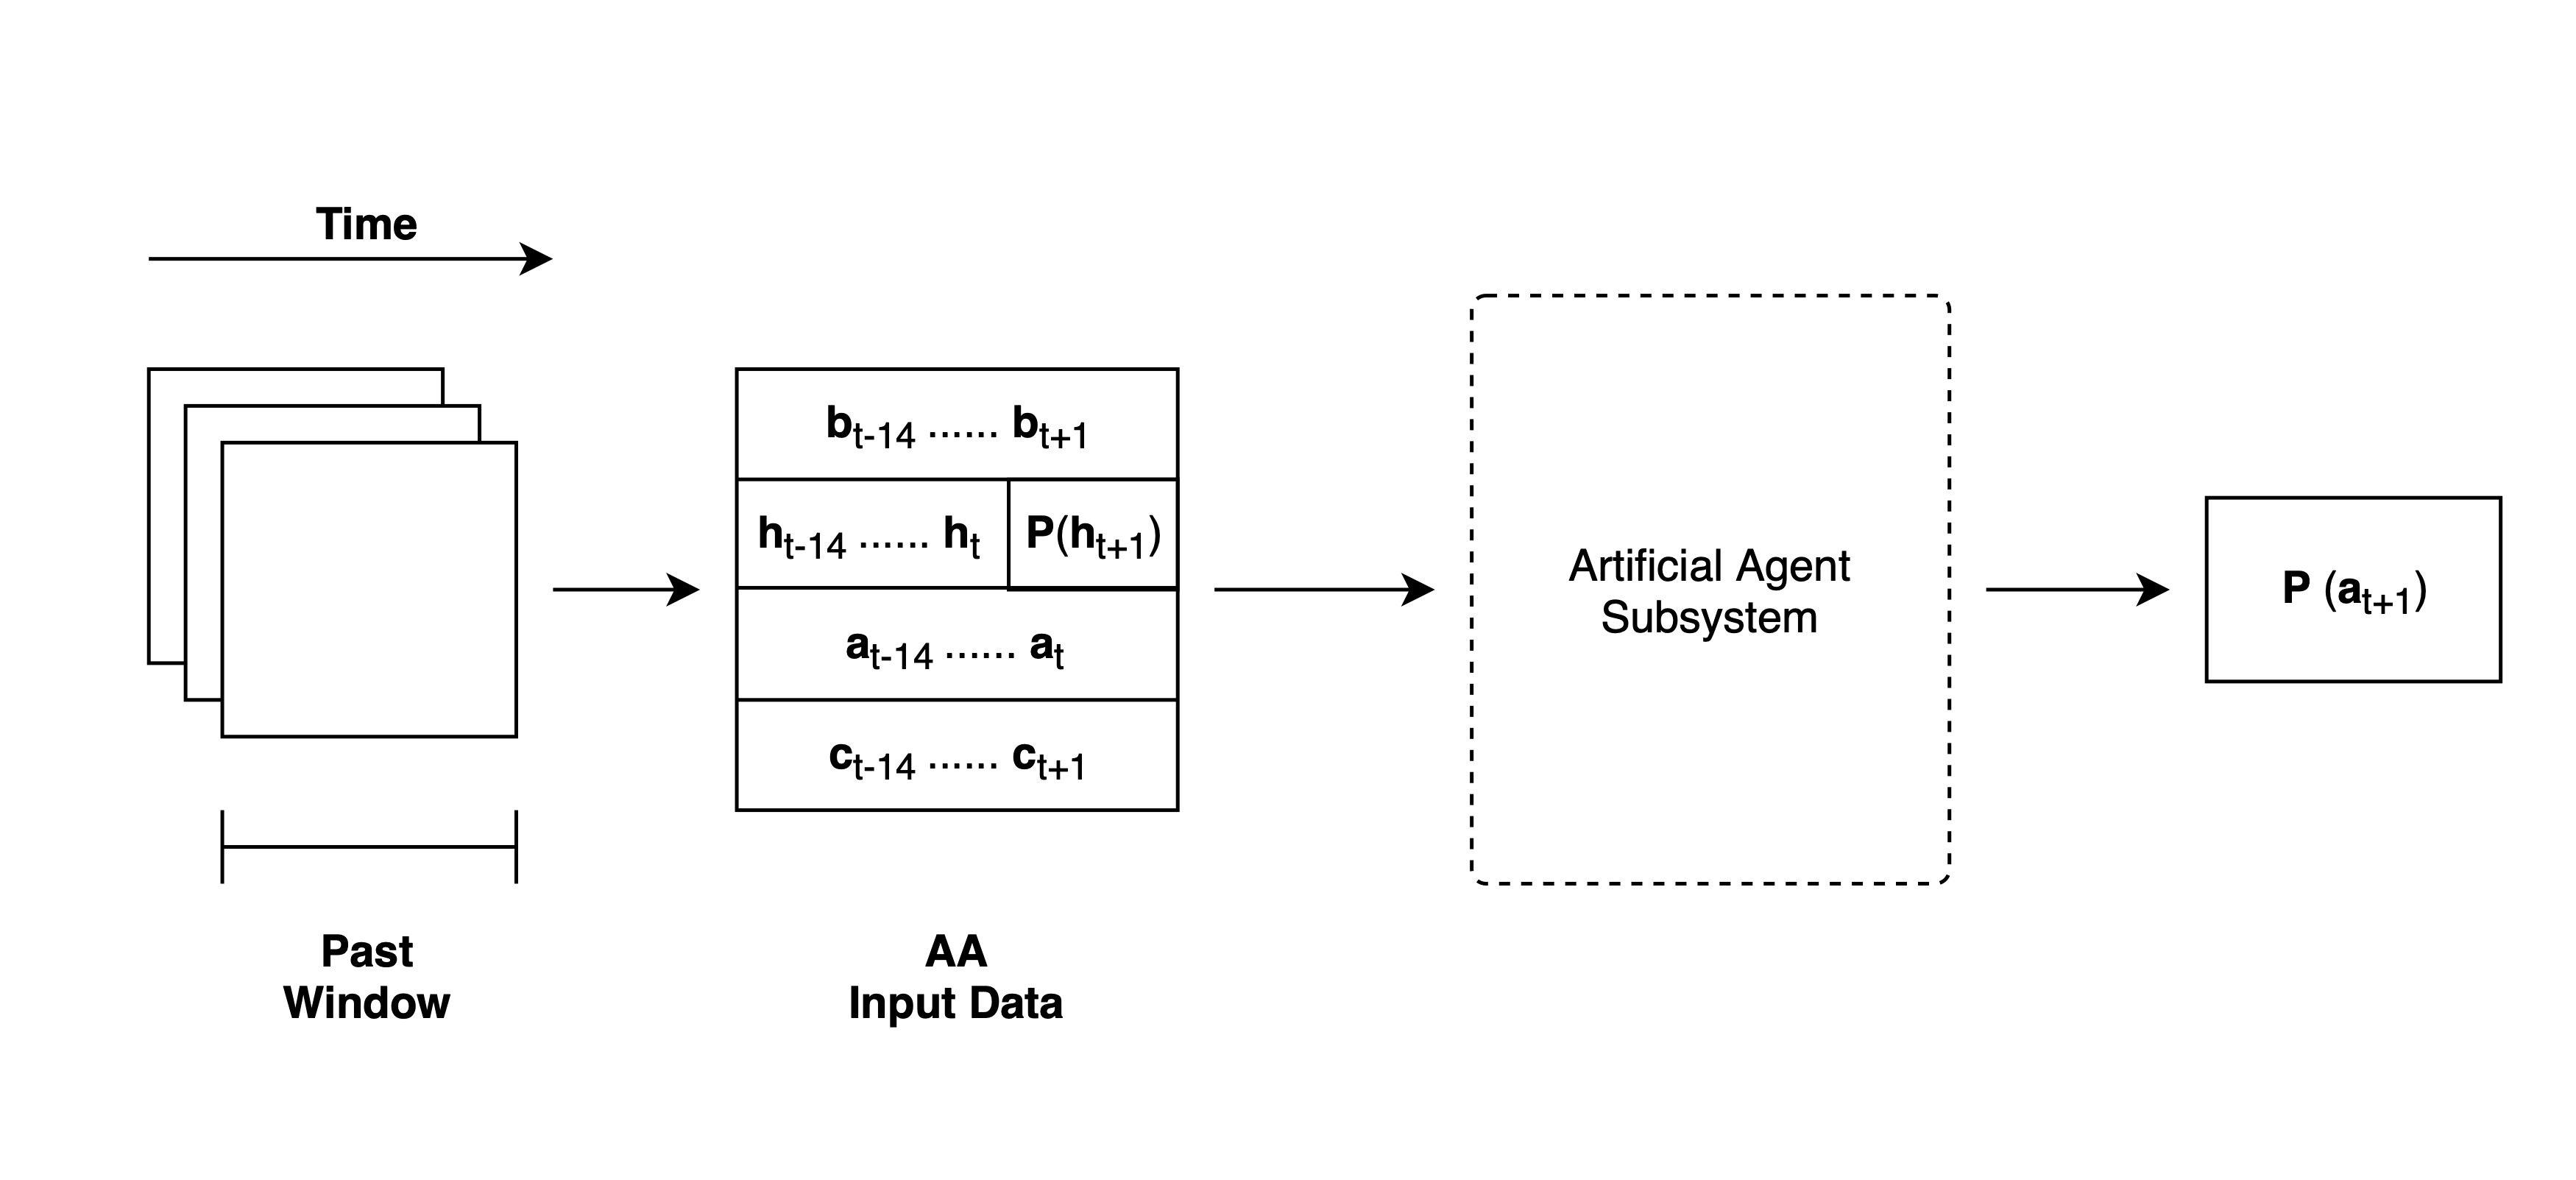
\includegraphics[width=0.8\textwidth]{media/aa_overall.jpg}
        \caption{The Artificial Agent Subsystem}
        \label{fig:aa_architecture}
        \end{figure}


        \subsection{Training}
        The system was trained for approximately 1200 epochs, with a batch size of 128 samples.  For the minimization of the categorical cross-entropy cost function, the Adam\textsuperscript{\cite{adam2014}} optimisation algorithm was used, with the learning rate set to 0.001 . The average time of the overall system's prediction was around 0.66 ms, 0.31 ms for the HA to predict the human solo and 0.35 ms for the AA to make the final prediction of the accompaniment chord. The loss of the training objective function in the validation set across the total epochs for which the models were trained, is shown in figure \ref{fig:val_loss}. 

        \begin{figure}[h]
        \centering
        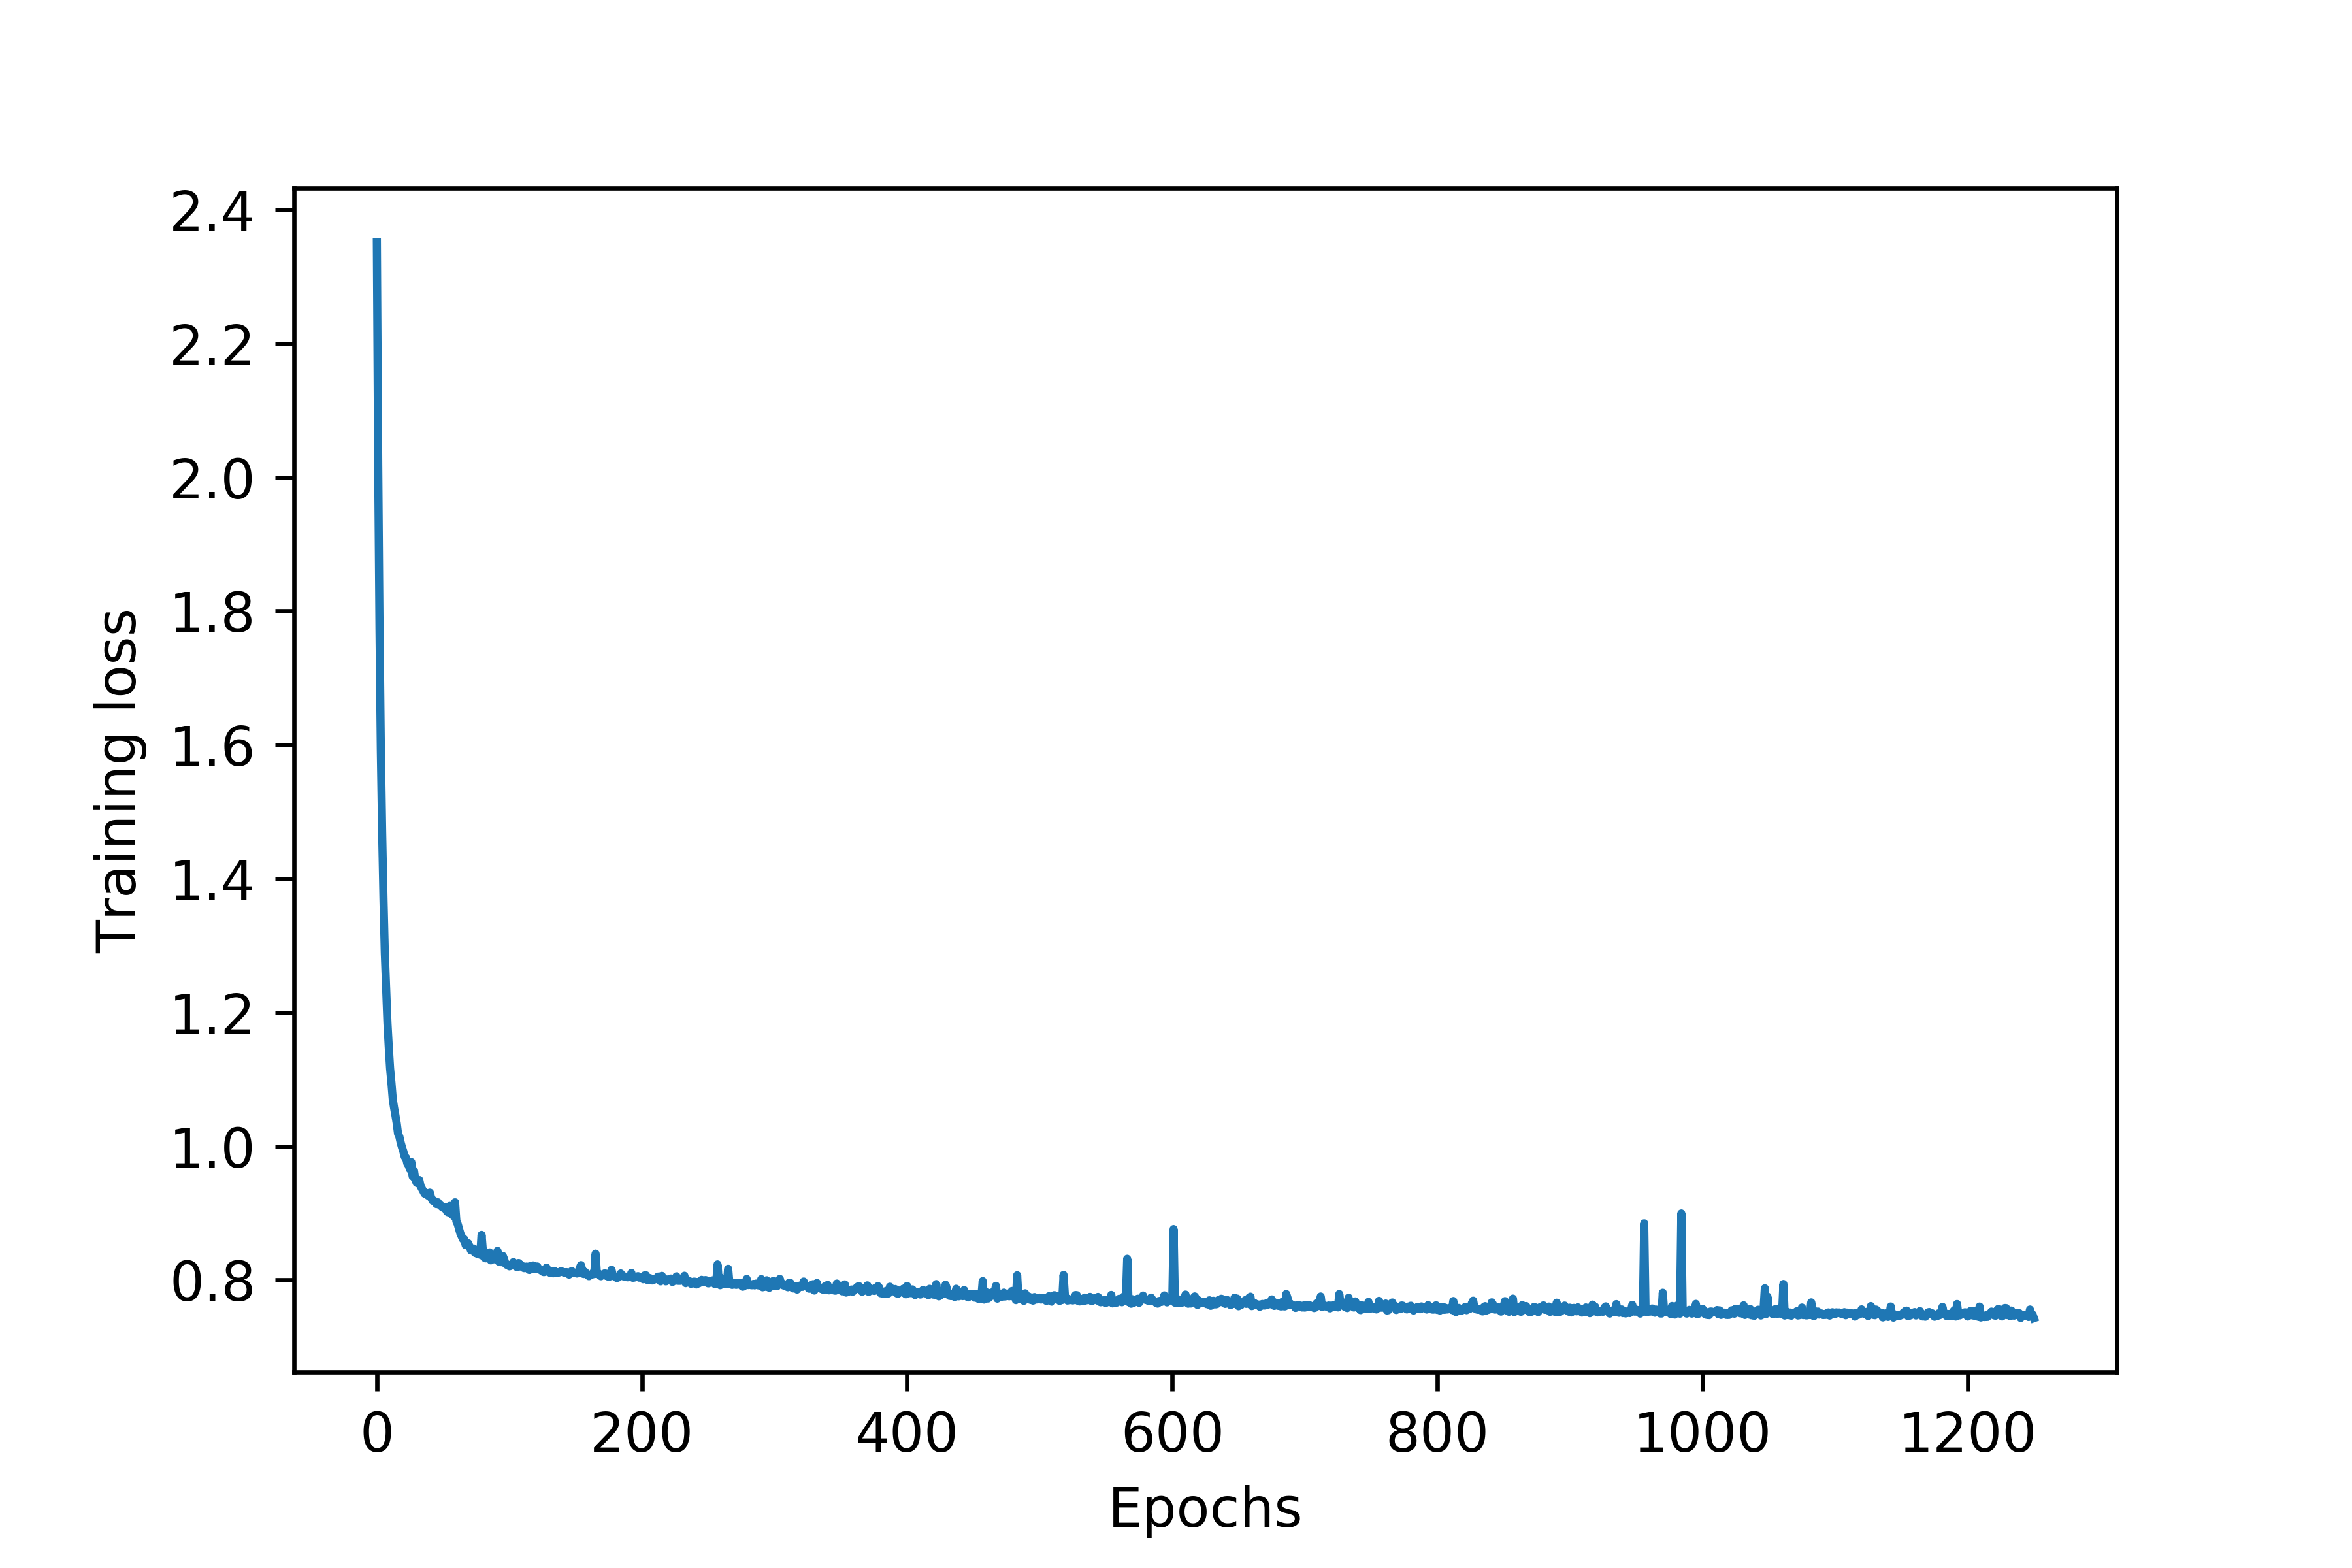
\includegraphics[width=0.65\textwidth]{media/epoch_val_loss_labels.png}
        \caption{Validation loss of the objective function over the total number of epochs of training}
        \label{fig:val_loss}
        \end{figure}

        \subsection{Real - Time Performance}
        A web application prototype has also been developed, based on MIDI.js and Tensorflow.js javascript libraries, aiming to test the degree in which the system is able to adapt to the solo input in a real time setting. 
    
        First, before the real-time performance, a number of measures to work on is defined as well as the metric structure and then the measures are filled with lead sheet chord information. The iterations are appointed by the metric structure, namely the duration of the measures (the amount of eighths they consist of). The interface developed for this task, saves the information added by the soloist, to feed the system after transforming it to a proper input representation.
        
        Each iteration deploys HA to predict human solo information of time-step $t+1$  ($P(h\textsubscript{t+1})$), being fed information about the past 16 time-steps ($[\ b\textsubscript{t-14}...b\textsubscript{t+1}\ ]$, $[\ h\textsubscript{t-15}...h\textsubscript{t}\ ]$, $[\ c\textsubscript{t-14}...c\textsubscript{t+1}\ ]$). The predicted output $P(h\textsubscript{t+1})$ is added to the data window of the AA, which will produce the accompaniment chord of time-step $t+1$ ($P(a\textsubscript{t+1})$), taking under account all the data features during the past 16 steps ($[\ b\textsubscript{t-14}...b\textsubscript{t+1}\ ]$, $[\ h\textsubscript{t-14}...h\textsubscript{t}\ P(h\textsubscript{t+1})\ ]$, $[\ a\textsubscript{t-15}...a\textsubscript{t}\ ]$, $[\ c\textsubscript{t-14}...c\textsubscript{t+1}\ ]$). After the produced accompaniment is played along with the soloist's input ($h\textsubscript{t+1}$), the predicted output $P(a\textsubscript{t+1})$ and the real-time inserted human solo information $h\textsubscript{t+1}$ are saved to the data used as the system's input, to keep them as the accompanying and human solo information of that specific future time-step $t+1$, respectively. 

    